\subsection{Самодополнительные графы}

\begin{wrapfigure}{r}{0.25\textwidth}
    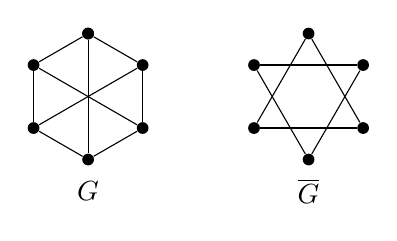
\begin{tikzpicture}[scale=0.8]
    % Первый граф (G)
    \begin{scope}[xshift=0cm]
        \foreach \angle [count=\i] in {90,150,...,450} {
            \node[circle, fill=black, inner sep=1.5pt] (v\i) at (\angle:1) {};
        }
        \foreach \i in {1,...,6} {
            \pgfmathtruncatemacro{\next}{mod(\i,6)+1}
            \draw (v\i) -- (v\next);
        }
        \draw (v1) -- (v4);
        \draw (v2) -- (v5);
        \draw (v3) -- (v6);
        \node at (0,-1.5) {$G$};
    \end{scope}
    
    % Второй граф (G с чертой)
    \begin{scope}[xshift=3.5cm]
        \foreach \angle [count=\i] in {30,90,...,389} {
            \node[circle, fill=black, inner sep=1.5pt] (w\i) at (\angle:1) {};
        }
        \foreach \i/\j in {1/3,3/5,5/1,2/4,4/6,6/2} {
            \draw (w\i) -- (w\j);
        }
        \node at (0,-1.5) {$\overline{G}$};
    \end{scope}
    \end{tikzpicture}
\end{wrapfigure}

\noindent\textbf{Определение.} \textit{Дополнение графа} $\overline{G}$ (граф с теми же вершинами, но противоположными связями):
\begin{itemize}[noitemsep,topsep=0pt]
\item Множество вершин: $V(\overline{G}) = V(G)$
\item Две вершины смежны в $\overline{G}$ $\Leftrightarrow$ несмежны в $G$
\end{itemize}

\noindent\textbf{Определение.} \textit{Самодополнительный граф} -- граф, изоморфный своему дополнению (структура графа совпадает со структурой его дополнения).

\noindent\textbf{Полный граф} $K_p$ (все вершины попарно соединены):
\begin{itemize}[noitemsep,topsep=0pt]
\item Содержит $p$ вершин
\item Имеет $\binom{p}{2}$ рёбер
\item Является регулярным степени $p-1$
\item Частный случай: $K_3$ -- треугольник
\end{itemize}

\noindent\textbf{Вполне несвязный граф} $\overline{K_p}$ -- дополнение полного графа (регулярный граф степени 0).